
Pour mesurer le pourcentage de cases corrig\'es, nous allons proc\'eder comme suit :
\begin{enumerate}[label = (\alph*)]
	\item Consid\'erer les cases {\em fausses positives} dans la matrice $M_s$ puis repr\'esenter le nombre de cases {\em fausses positives} pour chaque valeur de seuil. 
	Le graphique $(a)$ de la figure \ref{graphiquesFctCoutNormale} correspond \`a  la comparaison des seuils par rapport au nombre de cases {\em fausses positives} avant la correction.
	Nous remarquons qu'il n'y a aucune case {\em fausse positive} dans $M_s$ pour $s\in\{0.8,0.9\}$. Ce nombre croit quand le seuil $s$ decroit ($s \rightarrow 0$).
	
	\item Consid\'erer les cases {\em fausses n\'egatives} dans la matrice $M_s$ puis repr\'esenter le nombre de cases {\em fausses n\'egatives} pour chaque valeur de seuil.  Le graphique $(b)$ de la figure \ref{graphiquesFctCoutNormale}  correspond \`a la comparaison des seuils par rapport au nombre de cases {\em fausses n\'egatives} avant la correction. Le nombre des cases {\em fausses n\'egatives} est nul pour $s \not \in \{0.8,0.9\}$. 

	\item Consid\'erer les cases {\em fausses positives} apr\`es la correction de $G_s$ (matrice $M'_s$) puis repr\'esenter le nombre de cases {\em fausses positives} pour chaque valeur de seuil. Le graphique $(c)$ de la figure \ref{graphiquesFctCoutNormale} correspond \`a  la comparaison des seuils par rapport au nombre de cases {\em fausses positives} apr\`es la correction.
	 Le nombre de cases baisse quand $s \le 0.7$ puis augmente $s>0.7$.
	 
	\item Consid\'erer les cases {\em fausses n\'egatives} apr\`es la correction de $G_s$ (matrice $M'_s$) puis repr\'esenter le nombre de cases {\em fausses n\'egatives} pour chaque valeur de seuil. Le graphique $(d)$ de la figure \ref{graphiquesFctCoutNormale} correspond \`a la comparaison des seuils par rapport au nombre de cases {\em fausses n\'egatives} apr\`es la correction. Le nombre de cases varie peu quand $s < 0.4$ puis baisse quand $s = \{0.5, 0.6\}$ avant d'atteindre sa valeur minimum \`a $s = 0.7$. Il augmente $s>0.7$.
	
	\item Repr\'esenter les distances de Hamming moyennes de chaque graphe pour chaque seuil. Le graphique $(e)$ de la figure \ref{graphiquesFctCoutNormale} correspond \`a la comparaison des seuils en fonction de la distance de Hamming de chaque seuil.
	La distance de Hamming baisse quand $s \rightarrow 0.7$ avec sa valeur minimum \`a $s = 0.7$ puis augmente quand $s > 0.7$. 
\end{enumerate}
Rappelons que les diff\'erents graphiques sont rang\'es par ordre croissant et 
les distances de Hamming sont obtenues \`a partir la fonction de co\^ut {\em normale}.

Nous distinguons trois familles de seuils:
\begin{itemize}
	\item Les seuils $s < 0.7$ qui baissent le nombre de cases  {\em fausses positives} et augmentent celui des cases {\em fausses n\'egatives} apr\`es l'algorithme de correction. 
	Ils n'ont pas d'effets r\'eels sur la distance de Hamming car il y a un transfert d'\'el\'ements de l'ensemble des cases   {\em fausses positives} \`a celui des {\em fausses n\'egatives} et vice-versa. 
	\`A cet effet, on remarque  qu'il y a $20\%$ de cases {\em fausses n\'egatives} apr\`es la correction alors qu'il n'en existait aucune case {\em fausse n\'egative} avant la correction. 
	Il en est de m\^eme avec les cases  {\em fausses positives}  dont le nombre diminue de $20\%$  \'egalement pendant la correction. Ces seuils n'ont aucune influence sur les cases erron\'ees.
	% -------- graphiquesFctCoutNormale ---------
\begin{figure}[htb!] 
\centering
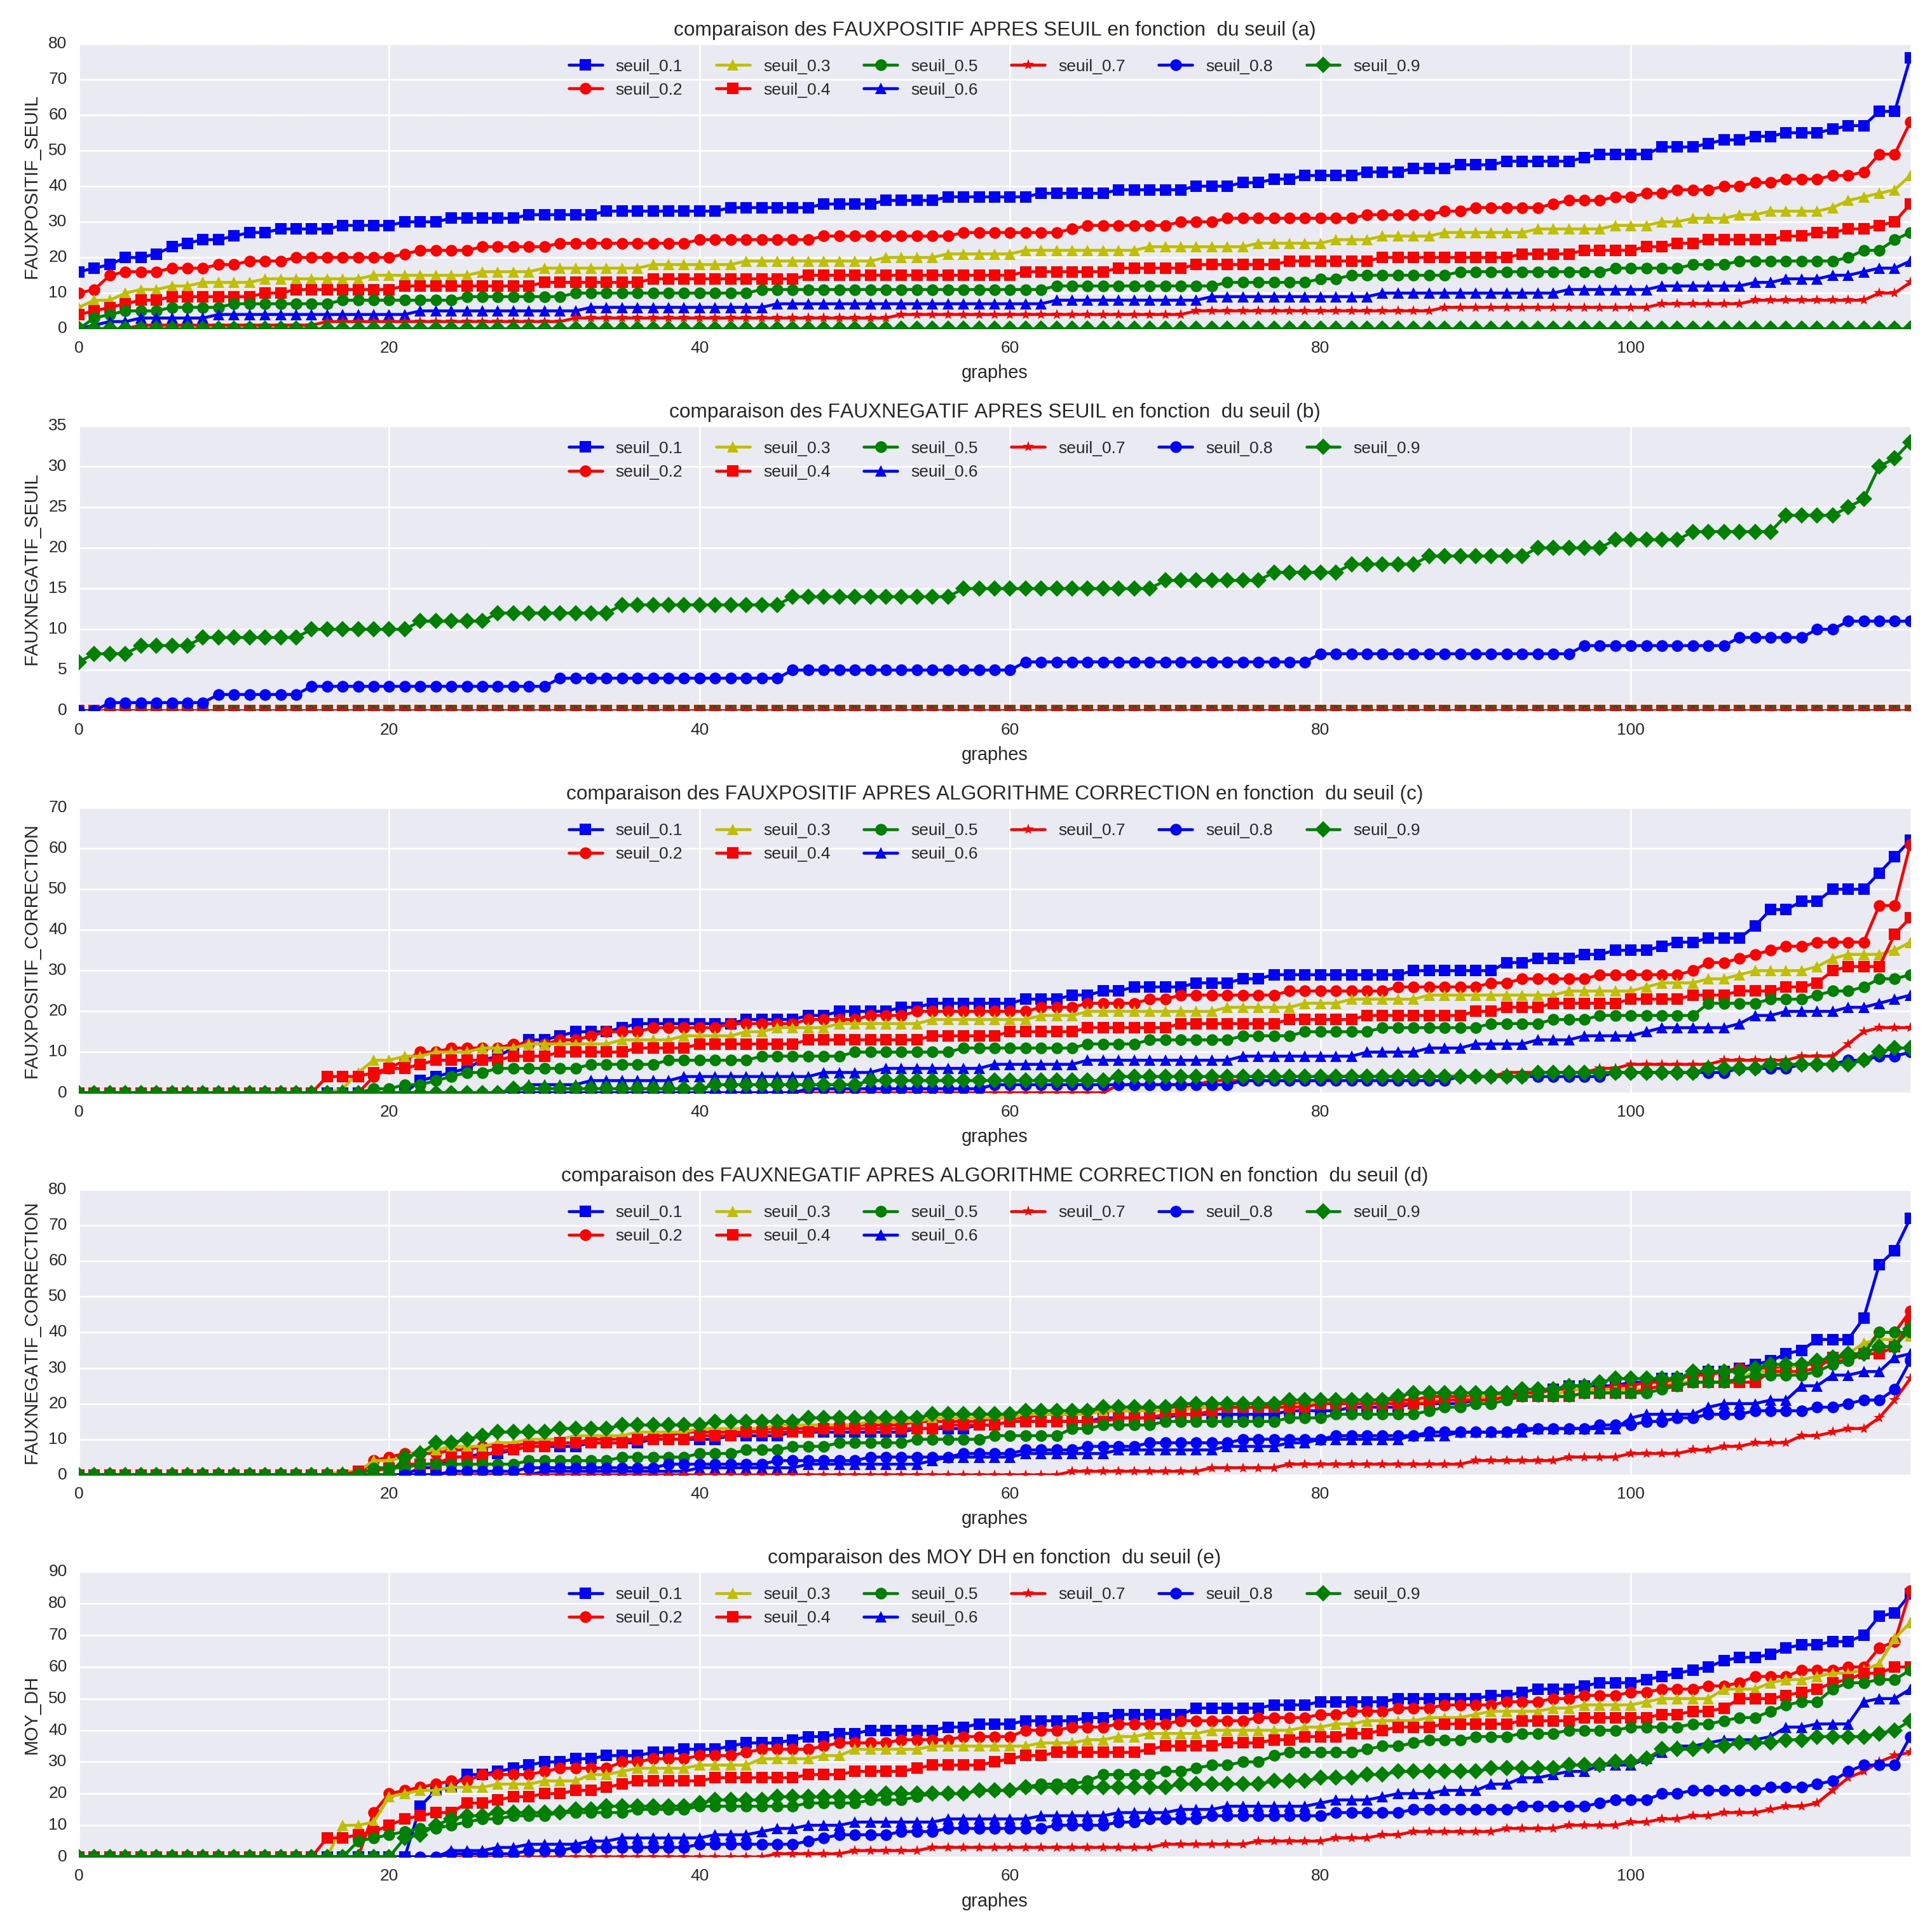
\includegraphics[scale=0.18]{choix_du_seuil_pour_fauxPositif_seuil_fauxNegatif_seuil_fauxPositif_correction_fauxNegatif_correction_moy_dh_aleatoire_normale.jpeg}
\caption{ Choix du seuil : (a) cases {\em fausses positives} dans la matrice $M_s$; (b) cases {\em fausses n\'egatives} dans la matrice $M_s$,(c) cases {\em fausses positives} dans la matrice $M'_s$; (d) cases {\em fausses n\'egatives} dans la matrice $M'_s$; (e) comparaison des seuils selon $moy\_DH$ }.
\label{graphiquesFctCoutNormale} 
\end{figure}
\FloatBarrier
% -------- graphiquesFctCoutNormale ---------

	\item Les seuils $s > 0.7$ qui augmentent le nombre de cases {\em fausses positives} et baissent celui des cases {\em fausses n\'egatives} apr\`es l'algorithme de correction. En effet, 
	le nombre de cases {\em fausses positives} est nul dans $M_s$ parce qu'il n'y a aucune case \`a $1$ ayant une valeur inf\'erieure \`a $s$ dans la distribution.
	Dans $M'_s$, le nombre moyen de cases {\em fausses positives} est de $1.76$ pour $s=0.8$ et de $2.33$ pour $s=0.9$. 
	Il y a l'ajout d'ar\^etes dans le graphe $LG_s$ parce que le nombre d'ar\^etes \`a supprimer pour corriger un sommet est tr\`es \'elev\'e et cela implique que le co\^ut de la correction par la suppression d'ar\^etes est tr\`es on\'ereux par rapport \`a celui de l'ajout d'ar\^etes. 
	Ainsi \`a chaque sommet \`a corriger, l'algorithme ajoute plus d'ar\^etes qu'il en supprime et certaines ar\^etes ajout\'ees appartiennent \`a l'ensemble des ar\^etes de $LG$.
	 Cela fait baisser les cases {\em fausses n\'egatives} comme nous le constatons avec les chiffres suivants : le nombre moyen de ces cases passe de  $6.7$ \`a $2.5$  pour $s = 0.8$ et de $17.7$ \`a $12.5$ pour $s = 0.9$.
	
	\item Le seuil $s=0.7$ qui diminue le nombre de cases {\em fausses n\'egatives} et {\em fausses positives}. En effet, le nombre moyen de cases erron\'ees est faible $< 10$ avant la phase de correction et il est $ \le 5$ apr\`es la correction. 
	Nous remarquons aussi les cases erron\'ees sont majoritairement des cases {\em fausses n\'egatives} apr\`es la correction.
	La pr\'esence de ces cases provient du co\^ut de modification des ar\^etes car la compression $\pi_1,\pi_2, \pi_s$ de co\^ut minimale n\'ecessite la suppression d'ar\^etes existantes.
	En effet, la matrice $M_s$ contient que des cases {\em fausses positives}. Pour trouver des bipartitions coh\'erentes (voir d\'efintion \ref{cliquesCoherentes}) autour des sommets \`a corriger, il faut ajouter beaucoup d'ar\^etes pour chaque partition et cela fait croitre le co\^ut de la correction. 
	Nous avons remarqu\'e aussi que la suppression de quelques ar\^etes permet d'obtenir des cliques qui correspondent \`a des sommets de $G$. L'algorithme pr\'ef\`ere alors supprimer des ar\^etes car elles sont peu par rapport aux ar\^etes \`a ajouter et aussi le co\^ut de la suppression d'ar\^etes est faible.
	 La distance de Hamming obtenue avec ce seuil est minimale par rapport aux autres seuils. Ce seuil fournit alors une meilleure correction des sommets de ${\cal C}$. 
	
\end{itemize}

{\bf Conclusion} : 
nous pouvons conclure que la repartition des cases erron\'ees avant la phase de correction a une influence sur l'algorithme de correction. 
Ainsi, le choix du seuil dans le bon intervalle permet de r\'eduire le nombre de cases erron\'ees et fournit une excellente correction des sommets de ${\cal C}$. 
Cependant,  les seuils diff\'erents du bon seuil  entraine que la fonction de co\^ut n'a aucune influence sur les corrections parce que l'algorithme corrige peu de cases erron\'ees mais ajoute aussi des cases {\em fausses positives} et {\em fausses n\'egatives} dans la m\^eme proportion. 

% ----------- comparaisonFctCoutUnitaireNormale -----------------
\begin{figure}[htb!] 
\centering
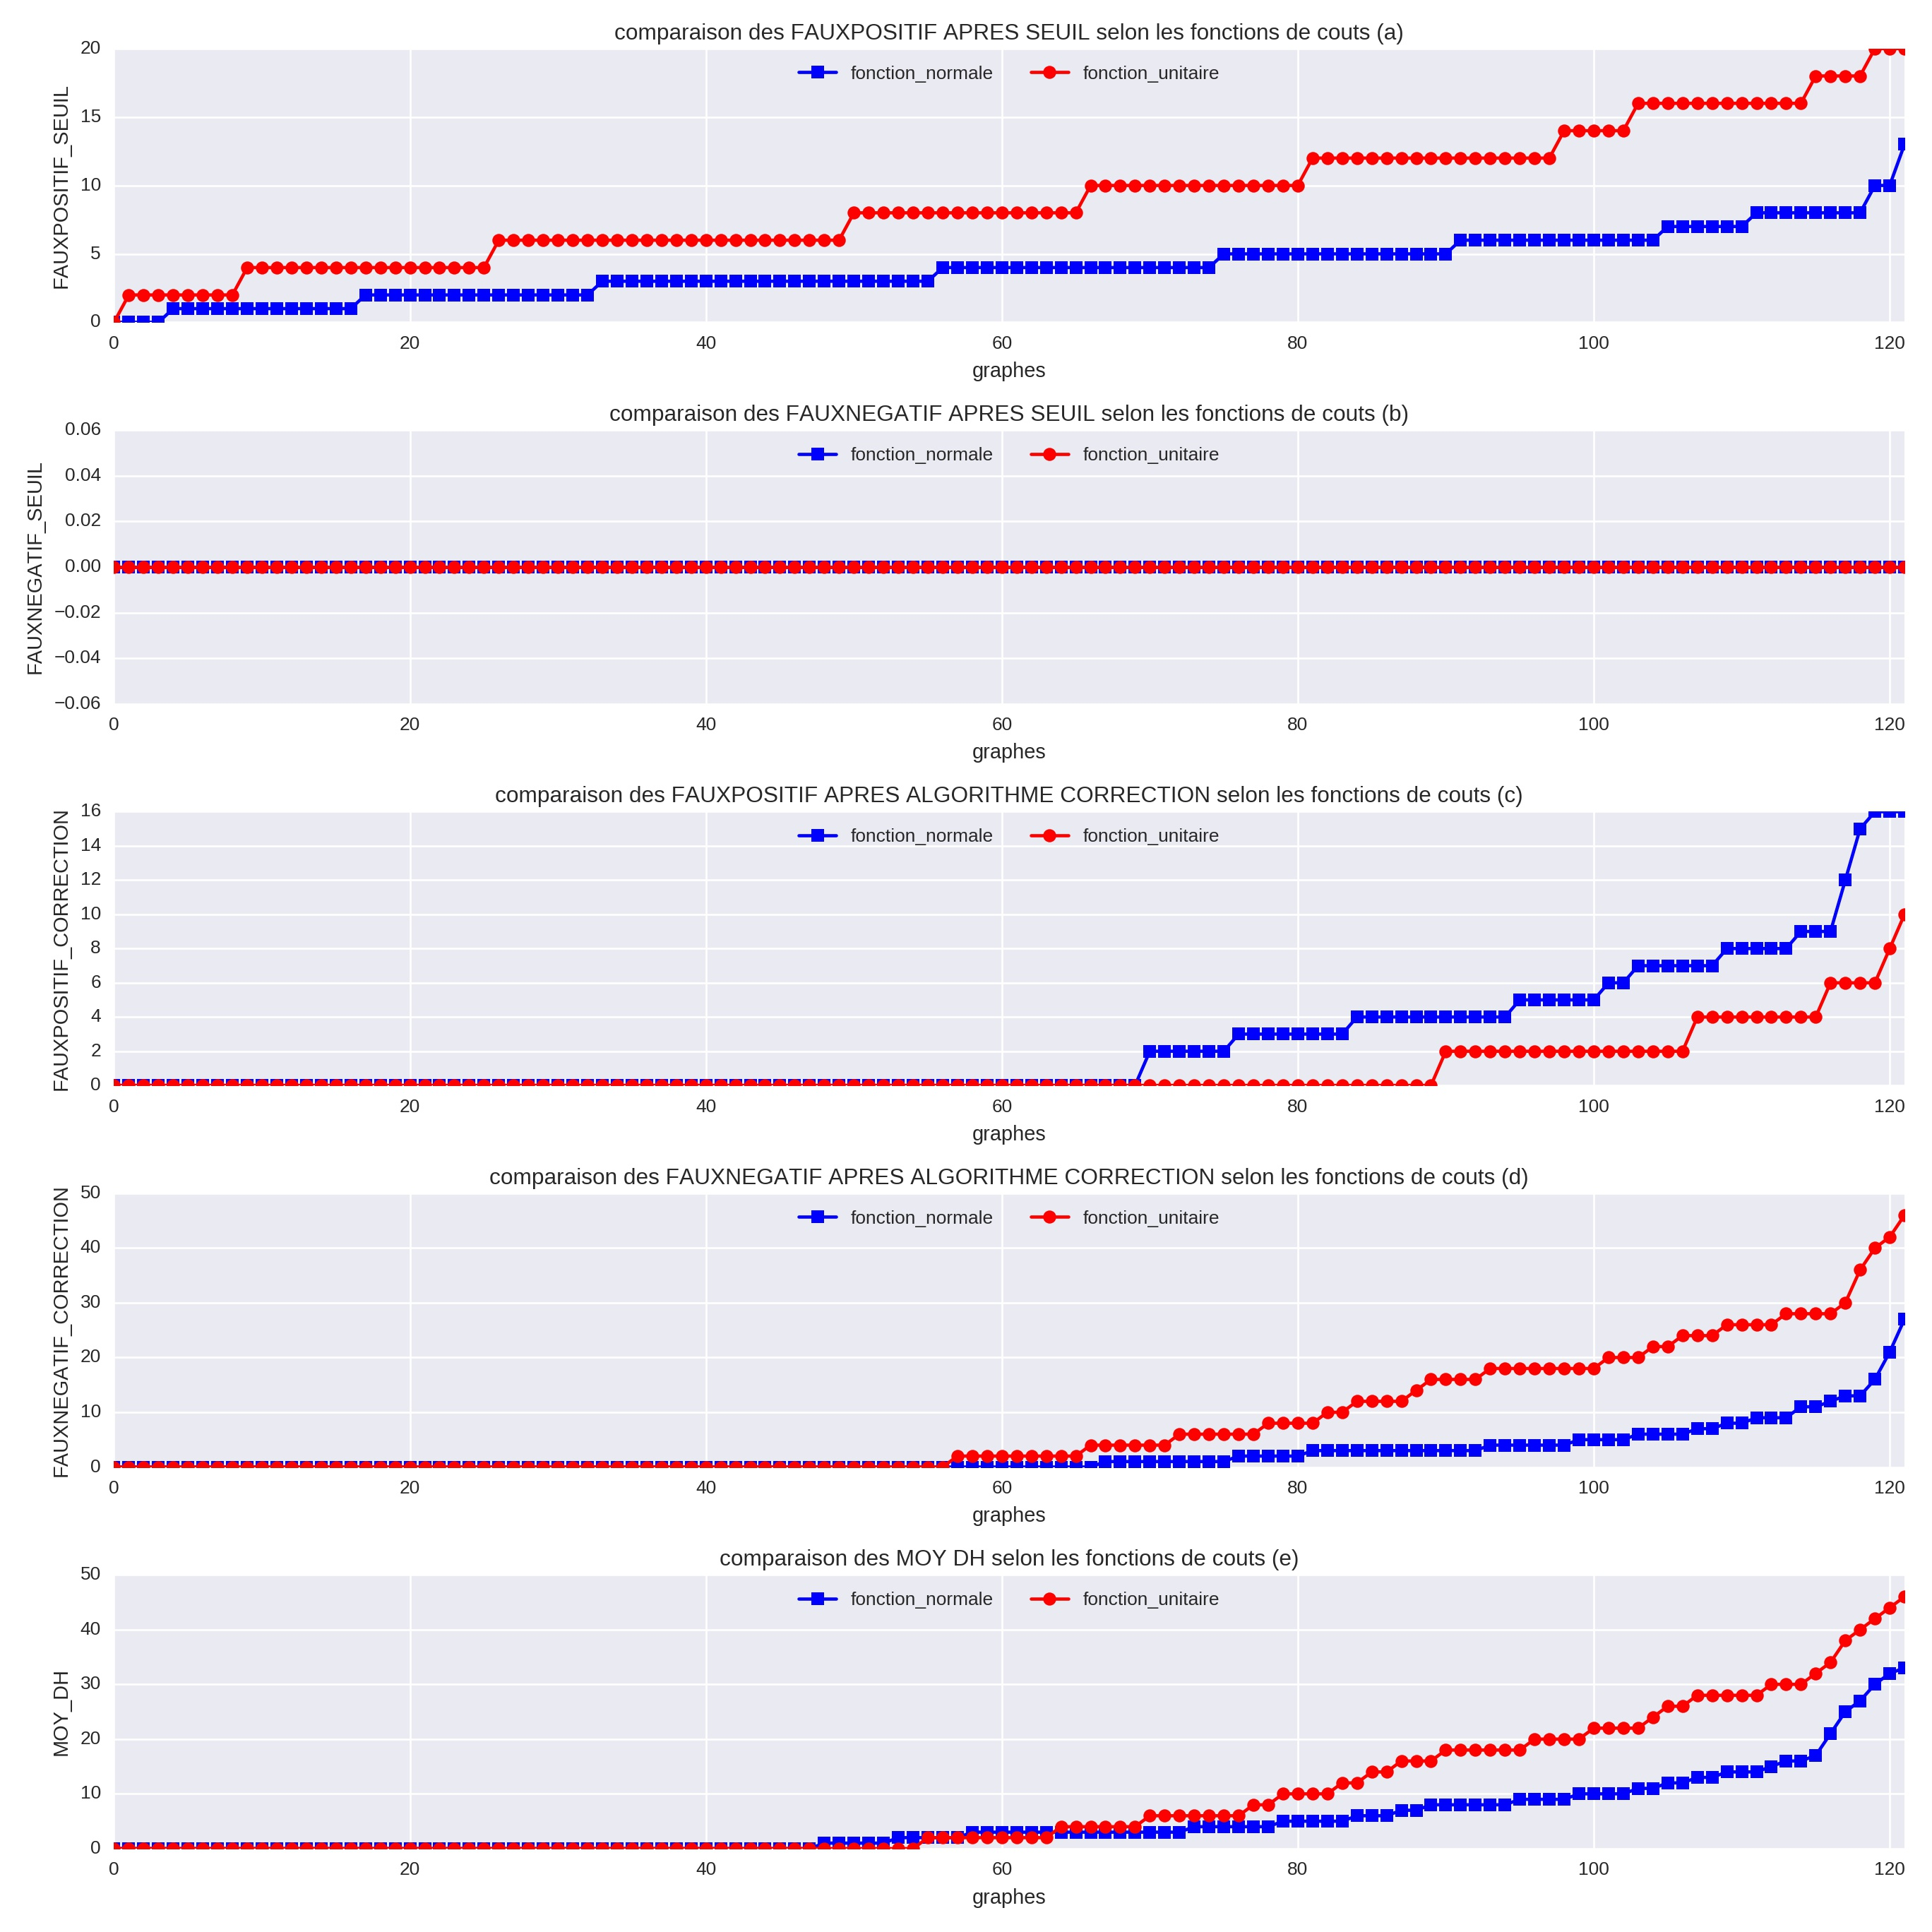
\includegraphics[scale=0.20]{choix_fct_cout_pour_fauxPositif_seuil_fauxNegatif_seuil_fauxPositif_correction_fauxNegatif_correction_moy_dh_aleatoire_s_07.jpeg}
\caption{ Comparaison entre les fonctions de co\^ut {\em unitaire} et {\em normale}: (a) cases {\em fausses positives} dans la matrice $M_s$; (b) cases {\em fausses n\'egatives} dans la matrice $M_s$; (c) cases {\em fausses positives} dans la matrice $M'_s$; (d) cases {\em fausses n\'egatives} dans la matrice $M'_s$; (e) comparaison des fonctions de co\^ut selon $moy\_DH$.}
\label{comparaisonFctCoutUnitaireNormale} 
\end{figure}
 \FloatBarrier
% ----------- comparaisonFctCoutUnitaireNormale -----------------

